%%% LaTeX Template: Designer's CV
%%%
%%% Source: http://www.howtotex.com/
%%% Feel free to distribute this template, but please keep the referal to HowToTeX.com.
%%% Date: March 2012


%%%%%%%%%%%%%%%%%%%%%%%%%%%%%%%%%%%%%
% Document properties and packages
%%%%%%%%%%%%%%%%%%%%%%%%%%%%%%%%%%%%%
\documentclass[a4paper,12pt,final]{memoir}

% misc
\renewcommand{\familydefault}{bch}	% font
\pagestyle{empty}					% no pagenumbering
\setlength{\parindent}{0pt}			% no paragraph indentation


% required packages (add your own)
\usepackage{flowfram}										% column layout
\usepackage[top=1cm,left=0.2cm,right=1cm,bottom=0.8cm]{geometry}% margins
\usepackage{graphicx}
\usepackage{epstopdf} 									% figures
\usepackage{url}											% URLs
\usepackage[usenames,dvipsnames]{xcolor}					% color
\usepackage{multicol}										% columns env.
	\setlength{\multicolsep}{1pt}
\usepackage{paralist}										% compact lists
\usepackage{tikz}
\usepackage{textcomp}

%\usepackage{anyfontsize}
\usepackage[hidelinks]{hyperref}

%%%%%%%%%%%%%%%%%%%%%%%%%%%%%%%%%%%%%
% Create column layout
%%%%%%%%%%%%%%%%%%%%%%%%%%%%%%%%%%%%%
% define length commands
\setlength{\vcolumnsep}{\baselineskip}
\setlength{\columnsep}{\vcolumnsep}

% frame setup (flowfram package)
% left frame
\newflowframe{0.265\textwidth}{\textheight}{0pt}{0pt}[left]
	\newlength{\LeftMainSep}
	\setlength{\LeftMainSep}{0.2\textwidth}
	\addtolength{\LeftMainSep}{4\columnsep}

% right frame
\newflowframe{0.7\textwidth}{\textheight}{\LeftMainSep}{0pt}[main01]

% horizontal rule between frames (using TikZ)
\renewcommand{\ffvrule}[3]{%
\hfill
\tikz{\draw[loosely dotted,color=Plum,line width=1.5pt,yshift=-#1](0, 0) -- (0pt,#3);}
\hfill\mbox{}}
\insertvrule{flow}{1}{flow}{2}


%%%%%%%%%%%%%%%%%%%%%%%%%%%%%%%%%%%%%
% define macros (for convience)
%%%%%%%%%%%%%%%%%%%%%%%%%%%%%%%%%%%%%
\newcommand{\Sep}{\vspace{1.5em}}
\newcommand{\SmallSep}{\vspace{0.5em}}

\newenvironment{Objective}
	{\ignorespaces\textbf{\color{Plum} Objective}}
	{\Sep\ignorespacesafterend}
	
\newcommand{\CVSection}[1]
	{\Large\textbf{#1}\par
	\SmallSep\normalsize\normalfont}

\newcommand{\CVItem}[1]
	{\textbf{\color{Plum} #1}}

%\urlstyle{}

%%%%%%%%%%%%%%%%%%%%%%%%%%%%%%%%%%%%%
% Begin document
%%%%%%%%%%%%%%%%%%%%%%%%%%%%%%%%%%%%%
\begin{document}

% Left frame
%%%%%%%%%%%%%%%%%%%%
%\begin{figure} 
%	\hfill
%	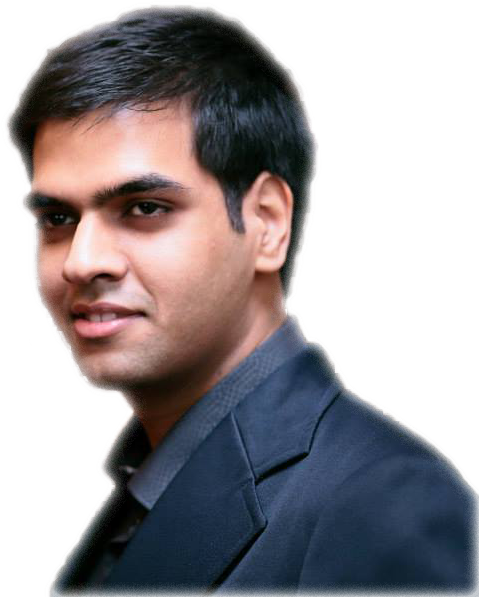
\includegraphics[width=0.8\columnwidth]{kkk}
%	\vspace{-5cm}
%\end{figure}

\begin{flushright} 
	\footnotesize
	\SmallSep
	{\bfseries{\color{Plum}{Address}}}\\
	
	2500, Avent Ferry Rd.\\
	Apartment No. 205\\
	Raleigh, NC - 27606\\
	\Sep
	{\bfseries{\color{Plum}{EMail}}}\\
	\href{mailto:vicky.p.katara@gmail.com}{vicky.p.katara@gmail.com}\\
	\Sep
	{\bfseries{\color{Plum}{Cellphone}}}\\
	\href{tel:+19842158067}{+1 984 215 8067}\\
	\Sep
		%{\bfseries{\color{Plum}{Website}}}\\
	%\href{http://vickykatara.orgfree.com/}{vickykatara.orgfree.com}\\
\end{flushright}\normalsize
%\begin{figure}
	%\hfill
	%\vspace{-0.3cm}
	\hspace{0.9cm}
		\vspace{-0.35cm}
	\bfseries{\color{Plum}{Save My Contact}}\\\\
	\vspace{-0.1cm}
	\hspace{-0.4cm}
	
\includegraphics[width=0.8\columnwidth]{qrcode_2.eps}
%\end{figure}
\framebreak

% Right frame
%%%%%%%%%%%%%%%%%%%%
\Huge\bfseries {\color{Plum} Vicky Katara} \\
\Large\bfseries  Computer Engineering Graduate \\

\normalsize\normalfont

% About me
\begin{Objective}
\\Achieve excellence in the field of Computer Science while refining the ability of visualization and rationality of thought.
\end{Objective}

% Education
\CVSection{Education}
\CVItem{2015 - 2017 (Expected), M.S.(Computer Science), North \hyphenchar\font=-1 Carolina State University}\\
\begin{footnotesize}
	Current GPA: Not available yet
\end{footnotesize}
\SmallSep

\CVItem{2009 - 2013, B.E.(Computer Engineering), University of \allowbreak  Mumbai}\\
 \begin{footnotesize}
 	Majored in Software / Computer Science. Minored in Computer Hardware / Electronics. Passed out with 72.46\%. Ranked 6 out of 130.
 \end{footnotesize}
\SmallSep

% Experience
\CVSection{Work Experience}
\CVItem{Jan 2014 \textendash \space Jun 2015, Technology Analyst, Deloitte Consulting}\\
\SmallSep
Information Management: Business Intelligence - Data Warehousing\\
\begin{minipage}{13cm}
\begin{compactitem}[\color{Plum}$\circ$]
	{\footnotesize
	\item Worked on a short term Data Integration project for one of the leading visualization software companies in the world
	\item Worked on a long term Enterprise Data Warehouse design and build project for one of the largest telecom service providers in the United States
	\item Worked on numerous firm and community improvement initiatives}
\end{compactitem}
\end{minipage}
\SmallSep\\
\CVItem{May 2006 \textendash \space present, Personal Tutor}\\
\SmallSep
Part time personal tutor to high school students\\
\begin{minipage}{13cm}
	\begin{compactitem}[\color{Plum}$\circ$]
		{\footnotesize
			\item Have taught more than 20 students, all between the ages of 14 and 19
			\item Subjects taught primarily include Mathematics and Physics}
	\end{compactitem}
\end{minipage}
\Sep

% Projects - Start
\CVSection{Projects}
%Project-4 Start
\CVItem{Analysis of Atomicity for Multithreaded Programs, B.E. Research Project}\\
{\footnotesize This involved research into algorithms for testing atomicity(serializability) of multi-threaded programs. The research was backed by a successful implementation to test the results.\\
	\emph{Technologies Used:} Java\texttrademark, Swing}%Project-4 End
\SmallSep\\
\CVItem{Design and Development of Acceleration Tool, Telecom Client}\\
{\footnotesize This tool would accept a batch of SQL Scripts via a Spreadsheet and execute them on an Oracle Database. It would then capture the resutls and publish it onto an Auditing and Testing platform.\\ \emph{Technologies Used:} Excel VBA
}	
\SmallSep\\
%Project-1 Start
\CVItem{Design and Development of Enterprise Data Warehousing, Telecom Client}\\
{\footnotesize The Data Warehouse was used as part of a Business Intelligence Suite which allowed the decision makers to monitor the sales and usage of products using Reporting Dashboards.\\ \emph{Technologies Used:} Informatica / Oracle, Unix, Tivoli Workload Scheduler
}	
\SmallSep\\
%Project-2 Start
\CVItem{Enterprise Data Integration, Visualization Software Client}\\
{\footnotesize This project involved enhancement and production support for the existing Enterprise Data Integration systems.\\ \emph{Technologies Used:} Informatica / Oracle, Unix}
\SmallSep\\
%Project-5 Start
%\CVItem{Development of Mini-Tennis Game, Mini-Project for Computer Graphics}\\
%{\footnotesize This involved the design and development of 2D Mini-Tennis game.\\ \emph{Technologies Used:} GCC}\\%Project-5 End
%\Sep 
% Projects - End
%%%%%%%%%%%%%%%%%%%%%%%%%%%%%%%%%%%%%
% End document
%%%%%%%%%%%%%%%%%%%%%%%%%%%%%%%%%%%%%
\end{document}